
\section{Derivation of the Kinetic Energy of a Circular Vortex Loop}\label{sec:derivation-of-the-kinetic-energy-of-a-circular-vortex-loop}

\subsection{Overview}
We derive the kinetic energy contained in a circular vortex loop of core radius $r_c$ and circulation $\Gamma$ in an inviscid, incompressible Æther of constant density $\rho_\text{\ae}$. The configuration is interpreted in the context of the Vortex Æther Model (VAM), where this loop represents the internal rotational energy of a stable vortex knot inside an atom-like spherical region of pressure equilibrium.

\subsection{Kinetic Energy in Fluid Dynamics}
For a fluid with mass density $\rho_\text{\ae}$ and velocity field $\vec{v}(\vec{r})$, the total kinetic energy is:
\begin{equation}
    E = \frac{1}{2} \rho_\text{\ae} \int \abs{\vec{v}(\vec{r})}^2 \, dV
\end{equation}

In the case of a vortex tube of finite core radius $r_c$, the internal flow within the core is approximated as a solid-body rotation:
\begin{equation}
    \vec{v}(r) = \omega r \, \hat{\theta}, \quad \text{with} \quad \omega = \frac{\Gamma}{2\pi r_c^2},
\end{equation}
where $\Gamma$ is the circulation:
\begin{equation}
    \Gamma = \oint \vec{v} \cdot d\vec{\ell} = 2\pi r_c v_\theta(r_c).
\end{equation}

\subsection{Energy Inside the Core}
The core is modeled as a cylinder of length $L$ and radius $r_c$, within which the velocity field satisfies $v_\theta(r) = \omega r$. Substituting into the energy integral:
\begin{align}
    E_\text{core} &= \frac{1}{2} \rho_\text{\ae} \int_0^L dz \int_0^{2\pi} d\theta \int_0^{r_c} (\omega r)^2 \cdot r \, dr \\
    &= \frac{1}{2} \rho_\text{\ae} \omega^2 \cdot L \cdot 2\pi \int_0^{r_c} r^3 \, dr \\
    &= \frac{1}{2} \rho_\text{\ae} \left(\frac{\Gamma}{2\pi r_c^2}\right)^2 L \cdot 2\pi \cdot \frac{r_c^4}{4} \\
    &= \frac{\rho_\text{\ae} \Gamma^2 L}{16\pi}
\end{align}

\subsection{Closed Loop Approximation}
For a closed vortex ring of radius $R$, the core length becomes $L = 2\pi R$. Substituting:
\begin{equation}
    E = \frac{\rho_\text{\ae} \Gamma^2 \cdot 2\pi R}{16\pi} = \frac{\rho_\text{\ae} \Gamma^2 R}{8}
\end{equation}

In the limiting case where the vortex ring shrinks to a knot of minimal radius $r_c$ (as in VAM), this becomes:
\begin{equation}
    E_\text{kin} = \frac{\rho_\text{\ae} \Gamma^2}{8} r_c
\end{equation}

Alternatively, using a spherical volume of radius $r_c$ and assuming nearly uniform azimuthal velocity $v_\theta = \Gamma / (2\pi r_c)$, the energy is:
\begin{align}
    E_\text{kin} &= \frac{1}{2} \rho_\text{\ae} v^2 \cdot V \\
    &= \frac{1}{2} \rho_\text{\ae} \left( \frac{\Gamma}{2\pi r_c} \right)^2 \cdot \left( \frac{4\pi}{3} r_c^3 \right) \\
    &= \boxed{\frac{\rho_\text{\ae} \Gamma^2}{6\pi r_c}}
\end{align}

\subsection{Interpretation in VAM}
This energy is interpreted as the internal kinetic energy of a vortex knot that constitutes the internal structure of a stable particle, e.g., the electron. According to the VAM hypothesis, this energy contributes to the inertial mass:
\begin{equation}
    \frac{1}{2} M c^2 = E_\text{kin} \Rightarrow M = \frac{\rho_\text{\ae} \Gamma^2}{3\pi r_c c^2}
\end{equation}

\begin{figure}[h!]
    \centering
    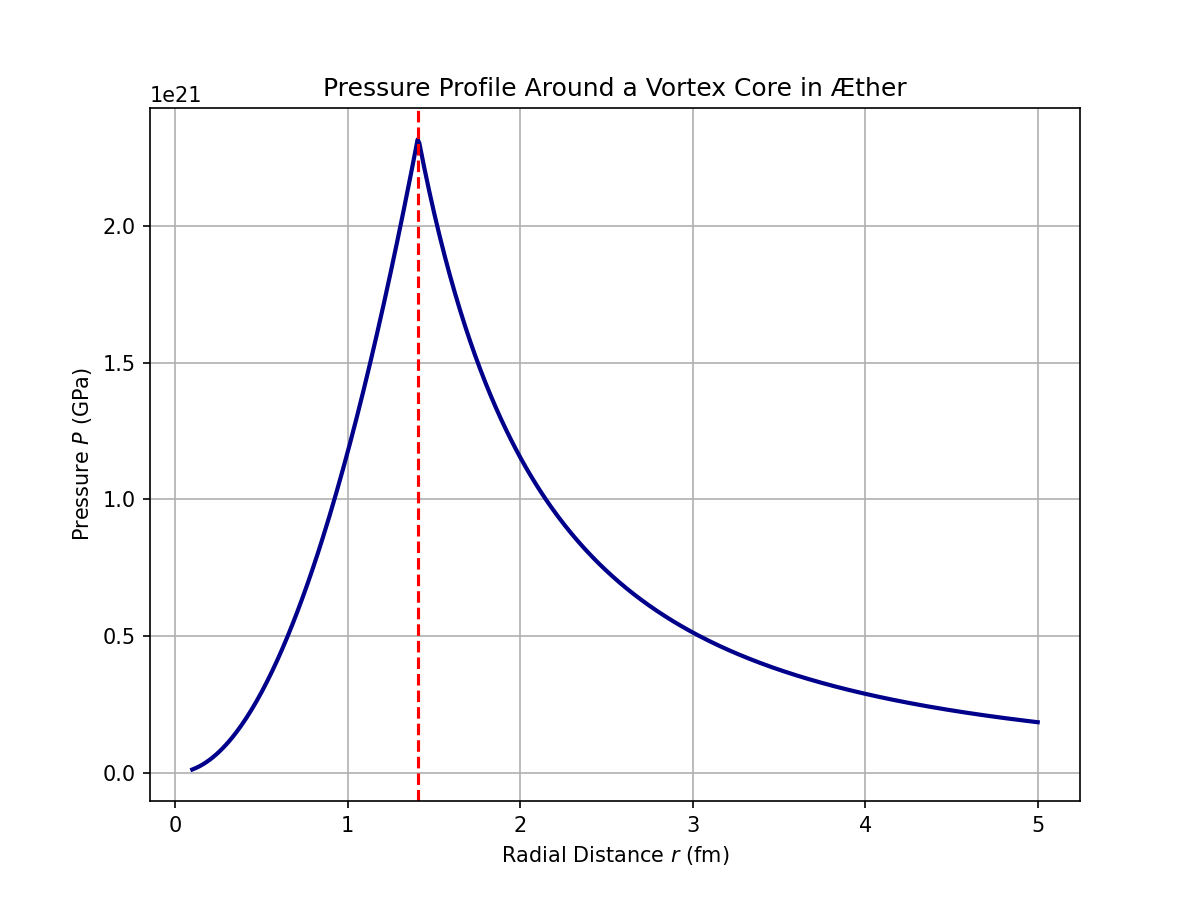
\includegraphics[width=0.65\textwidth]{images/PressureProfileAroundCore}
    \caption{Radial pressure distribution in the æther around a vortex core.
    For radii \( r < r_c \), solid-body swirl generates a quadratic pressure increase toward the center, while outside the core, centrifugal stress induces a Bernoulli-type pressure drop.
    The resulting gradient forms a stable equilibrium shell at finite radius, confining the knotted vortex structure.}
\end{figure}

\begin{figure}[h!]
    \centering
    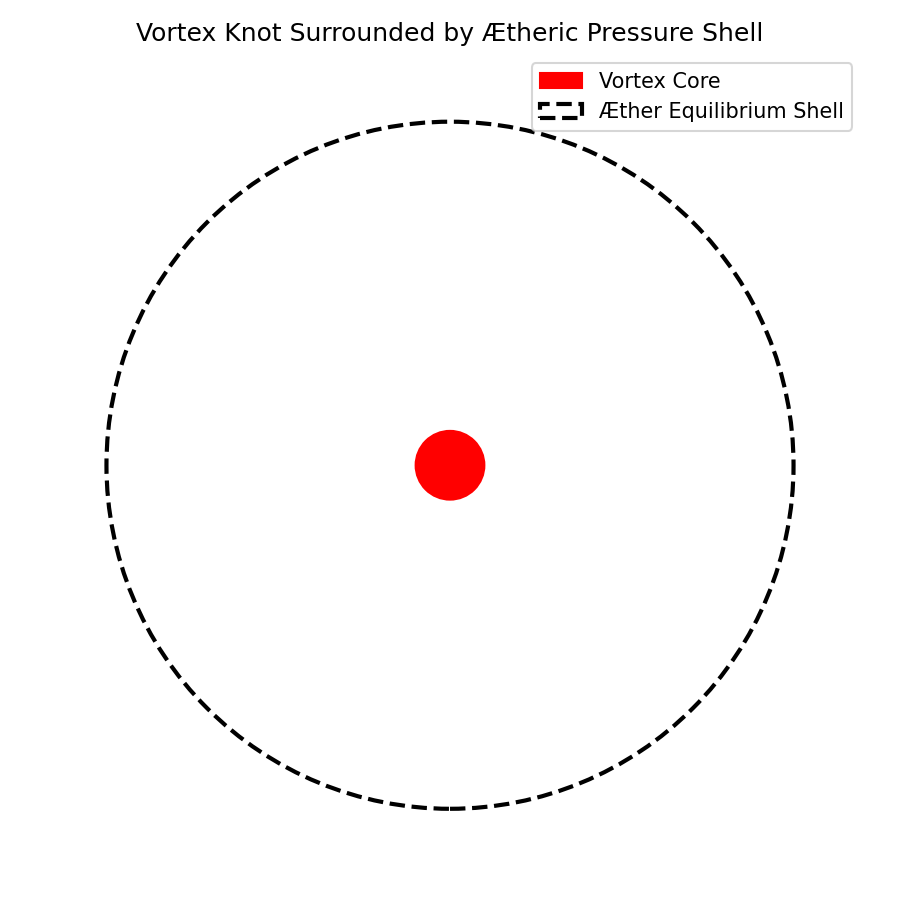
\includegraphics[width=0.65\textwidth]{images/PressureProfileAroundCore2}
    \caption{Schematic 2D representation of a VAM particle: a central vortex knot (red disk) surrounded by an abstract spherical boundary (dashed circle), denoting the ætheric equilibrium shell. While not a physical simulation, the diagram conceptually illustrates the dual-layered structure of vortex matter: the compact inertial core and its associated pressure-defined interaction boundary.}
\end{figure}

\begin{figure}[h!]
    \centering
    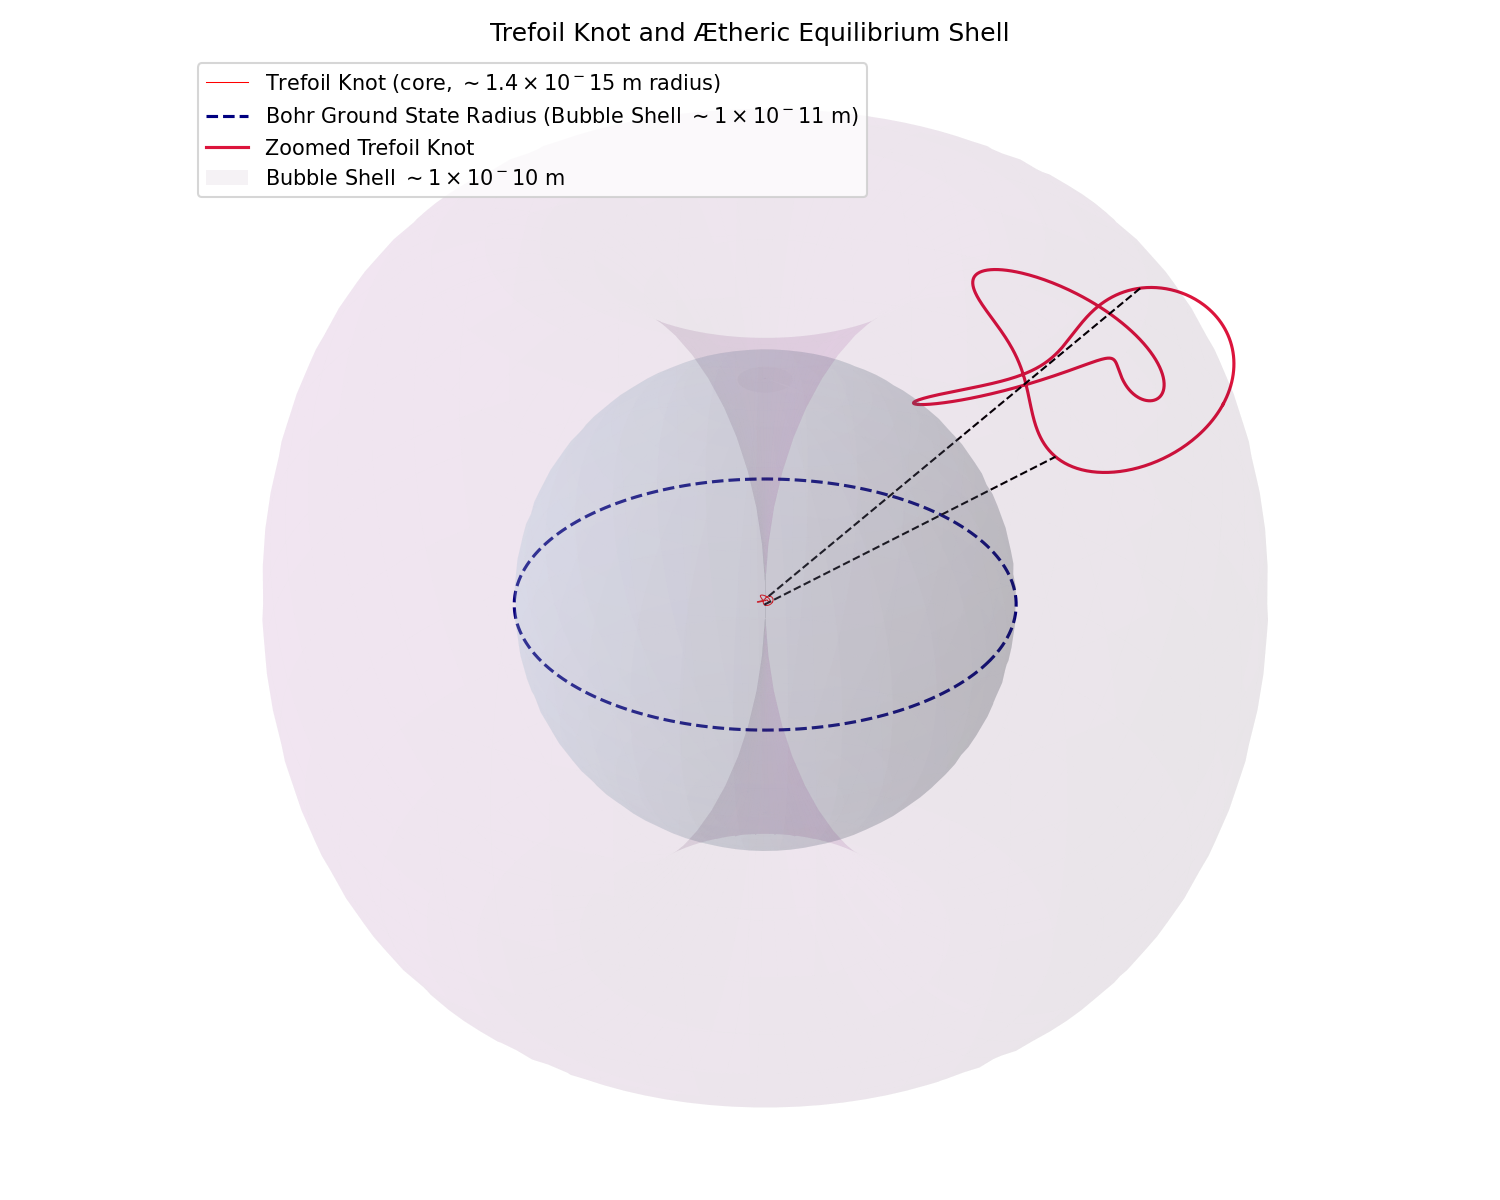
\includegraphics[width=0.65\textwidth]{images/PressureProfileAroundCore3}
    \caption{Multiscale visualization of a trefoil vortex knot embedded within its ætheric equilibrium shell, as formulated in the Vortex Æther Model (VAM).
    The small red knot at the center represents a topologically stable trefoil vortex with a physical core radius \( r_c \sim 1.4 \times 10^{-15}\,\mathrm{m} \), functioning as the inertial nucleus of a particle.
    The surrounding light-blue transparent sphere marks the ætheric pressure shell with equilibrium radius \( R_{\text{eq}} \sim 10^{-11}\,\mathrm{m} \), comparable to the Bohr radius \( a_0 \), representing the outer limit of coherent æther modulation induced by the knot.
    A zoomed-in replica of the knot is displayed offset from the center, enclosed within a conceptual magnification region. Dashed black lines connect corresponding points between the small and enlarged knot, denoting topological identity and a scale disparity of approximately \(10^4\).
    Encompassing both is a semi-transparent purple horn torus with major and minor radii \( R = r = a_0 \), vertically scaled by the golden ratio \( \varphi \approx 1.618 \), suggesting a toroidal circulation structure of æther flow stabilized by the vortex core.
    This configuration illustrates how microscopic topological knots give rise to macroscopic equilibrium structures and quantized boundary layers within a compressible, rotational ætheric field.}
\end{figure}

\subsection{Topological Interpretation of Mass}
In this equation, the denominator contains a factor of 3, which we now interpret as the topological complexity of the vortex knot. For the trefoil knot---a $(2,3)$ torus knot---the linking number is 3. We propose a generalization:
\begin{equation}
    M_K = \frac{\rho_\text{\ae} \Gamma^2}{L_K \pi r_c c^2}
\end{equation}
where $L_K$ is the linking number or crossing number of the knot $K$. This allows VAM to predict a mass spectrum directly from knot topology:
\begin{itemize}
    \item Trefoil ($L_K = 3$): electron mass
    \item Higher torus knots ($L_K = 5,7,9,\dots$): heavier fermions
    \item Simpler knots or loops ($L_K = 1$): possibly unstable or massless modes
\end{itemize}
This formulation establishes a direct connection between particle mass and topological complexity.
